% Created by tikzDevice version 0.10.1 on 2016-06-30 12:19:17
% !TEX encoding = UTF-8 Unicode
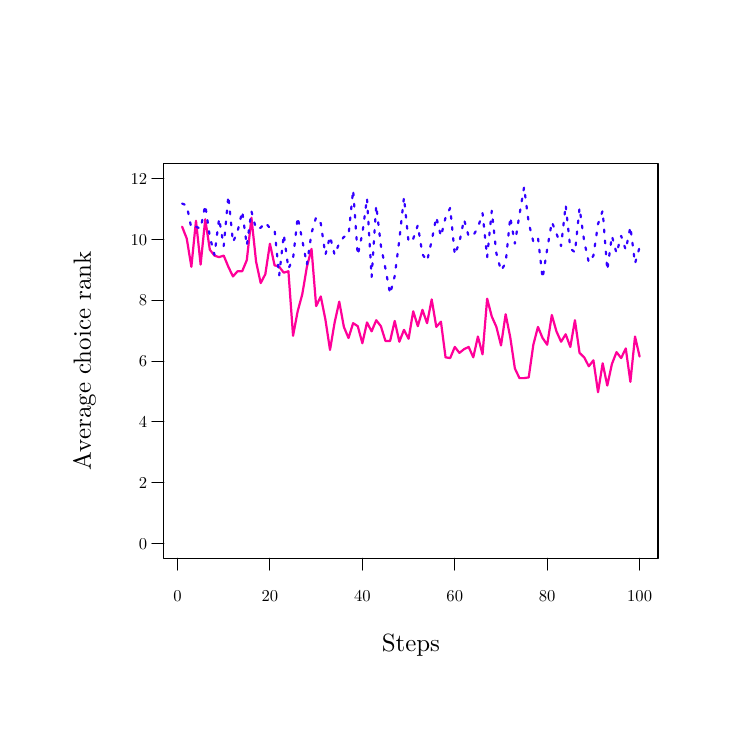
\begin{tikzpicture}[x=1pt,y=1pt]
\definecolor{fillColor}{RGB}{255,255,255}
\path[use as bounding box,fill=fillColor,fill opacity=0.00] (0,0) rectangle (252.94,252.94);
\begin{scope}
\path[clip] ( 49.20, 61.20) rectangle (227.75,203.75);
\definecolor{drawColor}{RGB}{255,0,153}

\path[draw=drawColor,line width= 0.8pt,line join=round,line cap=round] ( 55.81,181.03) --
	( 57.48,176.74) --
	( 59.15,166.54) --
	( 60.82,183.17) --
	( 62.49,167.35) --
	( 64.16,183.71) --
	( 65.83,172.71) --
	( 67.50,170.57) --
	( 69.17,170.03) --
	( 70.84,170.57) --
	( 72.51,166.54) --
	( 74.18,163.05) --
	( 75.85,164.93) --
	( 77.52,164.93) --
	( 79.19,168.96) --
	( 80.86,184.25) --
	( 82.53,168.42) --
	( 84.20,160.64) --
	( 85.87,163.86) --
	( 87.54,174.86) --
	( 89.21,167.08) --
	( 90.88,166.54) --
	( 92.55,164.40) --
	( 94.22,164.93) --
	( 95.89,141.59) --
	( 97.56,150.45) --
	( 99.23,156.62) --
	(100.90,166.54) --
	(102.57,172.98) --
	(104.24,152.32) --
	(105.91,155.81) --
	(107.58,147.50) --
	(109.25,136.50) --
	(110.92,146.42) --
	(112.59,153.93) --
	(114.26,144.81) --
	(115.93,140.79) --
	(117.60,146.15) --
	(119.27,145.08) --
	(120.94,138.91) --
	(122.61,146.42) --
	(124.28,143.20) --
	(125.95,147.23) --
	(127.62,145.08) --
	(129.29,139.72) --
	(130.96,139.72) --
	(132.63,146.96) --
	(134.30,139.45) --
	(135.97,143.74) --
	(137.64,140.52) --
	(139.31,150.45) --
	(140.98,145.08) --
	(142.65,150.98) --
	(144.32,146.15) --
	(145.99,154.74) --
	(147.66,144.81) --
	(149.33,146.69) --
	(151.00,133.81) --
	(152.67,133.55) --
	(154.34,137.57) --
	(156.01,135.42) --
	(157.68,136.76) --
	(159.35,137.57) --
	(161.02,133.81) --
	(162.69,141.33) --
	(164.36,134.89) --
	(166.03,155.01) --
	(167.70,148.57) --
	(169.37,144.81) --
	(171.04,138.11) --
	(172.71,149.37) --
	(174.38,141.06) --
	(176.05,129.79) --
	(177.71,126.30) --
	(179.38,126.30) --
	(181.05,126.57) --
	(182.72,138.37) --
	(184.39,144.81) --
	(186.06,140.79) --
	(187.73,138.37) --
	(189.40,149.10) --
	(191.07,143.20) --
	(192.74,139.45) --
	(194.41,142.13) --
	(196.08,137.57) --
	(197.75,147.23) --
	(199.42,135.42) --
	(201.09,133.81) --
	(202.76,130.59) --
	(204.43,132.74) --
	(206.10,121.21) --
	(207.77,131.67) --
	(209.44,123.62) --
	(211.11,131.40) --
	(212.78,135.69) --
	(214.45,133.55) --
	(216.12,137.03) --
	(217.79,124.96) --
	(219.46,141.33) --
	(221.13,134.08);
\end{scope}
\begin{scope}
\path[clip] (  0.00,  0.00) rectangle (252.94,252.94);
\definecolor{drawColor}{RGB}{0,0,0}

\path[draw=drawColor,line width= 0.4pt,line join=round,line cap=round] ( 54.14, 61.20) -- (221.13, 61.20);

\path[draw=drawColor,line width= 0.4pt,line join=round,line cap=round] ( 54.14, 61.20) -- ( 54.14, 56.92);

\path[draw=drawColor,line width= 0.4pt,line join=round,line cap=round] ( 87.54, 61.20) -- ( 87.54, 56.92);

\path[draw=drawColor,line width= 0.4pt,line join=round,line cap=round] (120.94, 61.20) -- (120.94, 56.92);

\path[draw=drawColor,line width= 0.4pt,line join=round,line cap=round] (154.34, 61.20) -- (154.34, 56.92);

\path[draw=drawColor,line width= 0.4pt,line join=round,line cap=round] (187.73, 61.20) -- (187.73, 56.92);

\path[draw=drawColor,line width= 0.4pt,line join=round,line cap=round] (221.13, 61.20) -- (221.13, 56.92);

\node[text=drawColor,anchor=base,inner sep=0pt, outer sep=0pt, scale=  0.60] at ( 54.14, 45.60) {0};

\node[text=drawColor,anchor=base,inner sep=0pt, outer sep=0pt, scale=  0.60] at ( 87.54, 45.60) {20};

\node[text=drawColor,anchor=base,inner sep=0pt, outer sep=0pt, scale=  0.60] at (120.94, 45.60) {40};

\node[text=drawColor,anchor=base,inner sep=0pt, outer sep=0pt, scale=  0.60] at (154.34, 45.60) {60};

\node[text=drawColor,anchor=base,inner sep=0pt, outer sep=0pt, scale=  0.60] at (187.73, 45.60) {80};

\node[text=drawColor,anchor=base,inner sep=0pt, outer sep=0pt, scale=  0.60] at (221.13, 45.60) {100};

\path[draw=drawColor,line width= 0.4pt,line join=round,line cap=round] ( 49.20, 66.48) -- ( 49.20,198.47);

\path[draw=drawColor,line width= 0.4pt,line join=round,line cap=round] ( 49.20, 66.48) -- ( 44.92, 66.48);

\path[draw=drawColor,line width= 0.4pt,line join=round,line cap=round] ( 49.20, 88.48) -- ( 44.92, 88.48);

\path[draw=drawColor,line width= 0.4pt,line join=round,line cap=round] ( 49.20,110.47) -- ( 44.92,110.47);

\path[draw=drawColor,line width= 0.4pt,line join=round,line cap=round] ( 49.20,132.47) -- ( 44.92,132.47);

\path[draw=drawColor,line width= 0.4pt,line join=round,line cap=round] ( 49.20,154.47) -- ( 44.92,154.47);

\path[draw=drawColor,line width= 0.4pt,line join=round,line cap=round] ( 49.20,176.47) -- ( 44.92,176.47);

\path[draw=drawColor,line width= 0.4pt,line join=round,line cap=round] ( 49.20,198.47) -- ( 44.92,198.47);

\node[text=drawColor,anchor=base east,inner sep=0pt, outer sep=0pt, scale=  0.60] at ( 43.20, 64.41) {0};

\node[text=drawColor,anchor=base east,inner sep=0pt, outer sep=0pt, scale=  0.60] at ( 43.20, 86.41) {2};

\node[text=drawColor,anchor=base east,inner sep=0pt, outer sep=0pt, scale=  0.60] at ( 43.20,108.41) {4};

\node[text=drawColor,anchor=base east,inner sep=0pt, outer sep=0pt, scale=  0.60] at ( 43.20,130.41) {6};

\node[text=drawColor,anchor=base east,inner sep=0pt, outer sep=0pt, scale=  0.60] at ( 43.20,152.40) {8};

\node[text=drawColor,anchor=base east,inner sep=0pt, outer sep=0pt, scale=  0.60] at ( 43.20,174.40) {10};

\node[text=drawColor,anchor=base east,inner sep=0pt, outer sep=0pt, scale=  0.60] at ( 43.20,196.40) {12};

\path[draw=drawColor,line width= 0.4pt,line join=round,line cap=round] ( 49.20, 61.20) --
	(227.75, 61.20) --
	(227.75,203.75) --
	( 49.20,203.75) --
	( 49.20, 61.20);
\end{scope}
\begin{scope}
\path[clip] (  0.00,  0.00) rectangle (252.94,252.94);
\definecolor{drawColor}{RGB}{0,0,0}

\node[text=drawColor,anchor=base,inner sep=0pt, outer sep=0pt, scale=  0.90] at (138.47, 27.60) {Steps};

\node[text=drawColor,rotate= 90.00,anchor=base,inner sep=0pt, outer sep=0pt, scale=  0.90] at ( 22.80,132.47) {Average choice rank};
\end{scope}
\begin{scope}
\path[clip] ( 49.20, 61.20) rectangle (227.75,203.75);
\definecolor{drawColor}{RGB}{51,0,255}

\path[draw=drawColor,line width= 0.8pt,dash pattern=on 1pt off 3pt ,line join=round,line cap=round] ( 55.81,189.39) --
	( 57.48,188.69) --
	( 59.15,180.48) --
	( 60.82,181.01) --
	( 62.49,180.31) --
	( 64.16,188.86) --
	( 65.83,177.34) --
	( 67.50,170.88) --
	( 69.17,183.98) --
	( 70.84,174.02) --
	( 72.51,192.18) --
	( 74.18,175.42) --
	( 75.85,179.26) --
	( 77.52,186.59) --
	( 79.19,174.20) --
	( 80.86,186.59) --
	( 82.53,180.13) --
	( 84.20,180.66) --
	( 85.87,182.58) --
	( 87.54,180.48) --
	( 89.21,179.96) --
	( 90.88,163.37) --
	( 92.55,178.21) --
	( 94.22,165.82) --
	( 95.89,169.48) --
	( 97.56,184.50) --
	( 99.23,176.12) --
	(100.90,167.39) --
	(102.57,178.74) --
	(104.24,184.50) --
	(105.91,182.23) --
	(107.58,170.88) --
	(109.25,177.52) --
	(110.92,170.88) --
	(112.59,175.07) --
	(114.26,177.34) --
	(115.93,177.86) --
	(117.60,194.28) --
	(119.27,170.71) --
	(120.94,178.56) --
	(122.61,191.31) --
	(124.28,162.85) --
	(125.95,188.69) --
	(127.62,174.20) --
	(129.29,165.82) --
	(130.96,156.74) --
	(132.63,163.20) --
	(134.30,176.29) --
	(135.97,191.66) --
	(137.64,175.42) --
	(139.31,176.64) --
	(140.98,181.53) --
	(142.65,171.06) --
	(144.32,168.61) --
	(145.99,175.94) --
	(147.66,184.50) --
	(149.33,177.52) --
	(151.00,184.32) --
	(152.67,187.82) --
	(154.34,170.88) --
	(156.01,175.42) --
	(157.68,183.63) --
	(159.35,177.52) --
	(161.02,177.86) --
	(162.69,180.66) --
	(164.36,185.90) --
	(166.03,170.01) --
	(167.70,186.77) --
	(169.37,171.40) --
	(171.04,165.12) --
	(172.71,167.91) --
	(174.38,184.50) --
	(176.05,174.90) --
	(177.71,185.37) --
	(179.38,195.32) --
	(181.05,182.40) --
	(182.72,175.59) --
	(184.39,177.17) --
	(186.06,162.33) --
	(187.73,172.98) --
	(189.40,182.75) --
	(191.07,178.56) --
	(192.74,174.02) --
	(194.41,188.86) --
	(196.08,173.15) --
	(197.75,171.75) --
	(199.42,187.82) --
	(201.09,175.77) --
	(202.76,168.09) --
	(204.43,170.53) --
	(206.10,182.05) --
	(207.77,186.77) --
	(209.44,165.29) --
	(211.11,177.69) --
	(212.78,171.40) --
	(214.45,177.69) --
	(216.12,172.63) --
	(217.79,181.01) --
	(219.46,167.74) --
	(221.13,173.67);
\end{scope}
\end{tikzpicture}
